\subsection{Temperature Sensor}

\begin{figure}[h!]
	\centering
 	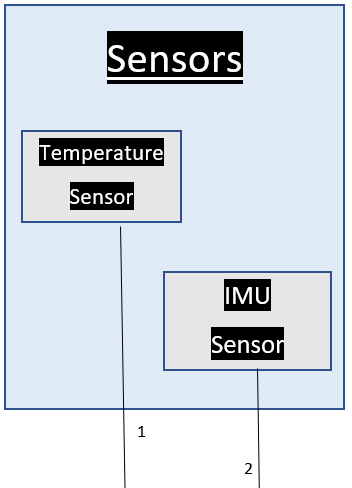
\includegraphics[width=0.60\textwidth]{images/Sensors subsystems}
 \caption{Sensor subsystems description}
\end{figure}

\subsubsection{Assumptions}
Temperature sensors are basically conducting metal having some resistance which can measure temperature in the form of electronic signal. Temperature sensor used in hydrometer has an accuracy of +- 1.5 degree C.

\subsubsection{Responsibilities}
It stores temperature in the form of  electronic signal and changes whenever the temperature changes.Temperature sensors only one function is to send the analog data of temperature to Arduino nano. 

\subsubsection{Subsystem Interfaces}
Each of the inputs and outputs for the subsystem are defined here. Create a table with an entry for each labelled interface that connects to this subsystem. For each entry, describe any incoming and outgoing data elements will pass through this interface.

\begin {table}[H]
\caption {Subsystem interfaces} 
\begin{center}
    \begin{tabular}{ | p{1cm} | p{6cm} | p{3cm} | p{3cm} |}
    \hline
    ID & Description & Inputs & Outputs \\ \hline
     & Temperature interface & \pbox{3cm}{N/A} & \pbox{3cm}{output 1}  \\ \hline
    \end{tabular}
\end{center}
\end{table}

\subsection{IMU Sensor}

\begin{figure}[h!]
	\centering
 	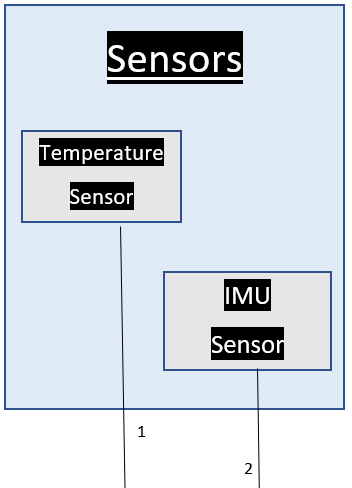
\includegraphics[width=0.60\textwidth]{images/Sensors subsystems}
 \caption{Sensor subsystems description}
\end{figure}

\subsubsection{Assumptions}

\subsubsection{Responsibilities}
Arduino nano 33 BLE is an advance microcontroller, it consists of 9-axis Inertial Measurement Unit (IMU) which refers to built in gyroscope, accelerometer and magnetometer. 

While floating, IMU send data to nano about it's position which is the primary function of IMU sensor. 


\subsubsection{Subsystem Interfaces}
Each of the inputs and outputs for the subsystem are defined here. Create a table with an entry for each labelled interface that connects to this subsystem. For each entry, describe any incoming and outgoing data elements will pass through this interface.

\begin {table}[H]
\caption {Subsystem interfaces} 
\begin{center}
    \begin{tabular}{ | p{1cm} | p{6cm} | p{3cm} | p{3cm} |}
    \hline
    ID & Description & Inputs & Outputs \\ \hline
     & IMU interface & \pbox{3cm}{N/A} & \pbox{3cm}{output 2}  \\ \hline
    \end{tabular}
\end{center}
\end{table}